The class diagram is a relational diagram between concepts that is closer to the implementation that the Domain Model. It tries to sketch a rough estemate about how the implementation could be realised. It has a great resemblance to object oriented programming since every class can be directly copied into code as a prototype for a future implementation.\\
The functions are derived from the white box sequence diagrams.\\
This class diagram is heavily based on relations, especially inheritance. Since our power tree is in essence an abstract simplified form of the class diagram. The primary goal is to have the user be the direct request parser for the interface. This ensures that any change in the kernel does not result in having to change the interface.\\
When the user authenticates itself, it is either staff or a member which we define as a (subclass of) Role, and attains the functions coming with that user class. This hides other functions that the user is not permitted to use, limiting the power to change the system to a minimum set of functions. As long as the user is permitted, it has access to 4 managers that are collections of (indirectly) all other classes.\\
All attributes are encapsulated. This is done by limiting the visibility to other classes. Functions are the only way to modify an instance of a class, and as we established, the functions available is limited to the role of the user.\\


Below is a set of support classes that are used to define groups of parameters. However, these are added just to simplify the function arguments and do not add any value.
\begin{figure}[H]
	\centering
	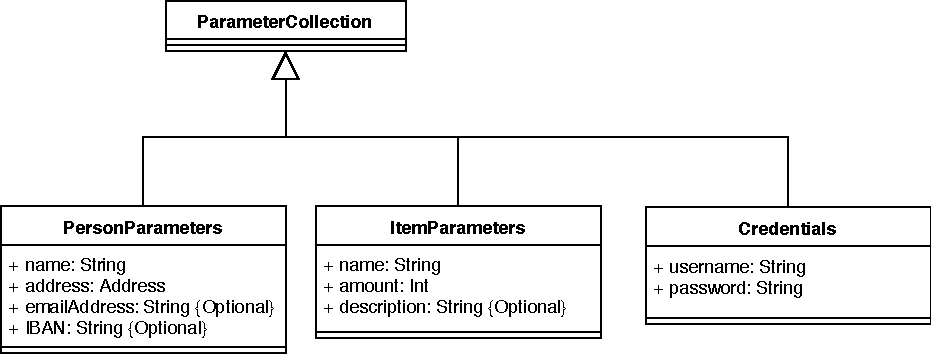
\includegraphics{uml/classdiagramsupport.pdf}
	\caption*{Some support classes for the class diagram}
\end{figure}